\documentclass{article}
\setlength{\parskip}{.5cm}
%\renewcommand{\thefigure}{\thesection.\arabic{figure}}
\usepackage[usenames,dvipsnames]{color}
\usepackage{lscape, graphicx}
\usepackage[colorlinks]{hyperref}
\usepackage{booktabs}
\usepackage[margin=1in]{geometry}
\bibliographystyle{acm}
\author{
{\small\textbf{Jesse Cook}}\\*
{\small Class: CS 525 - Principles of Simulation}\\*
{\small Professor: Dr. Mayer}
}
\title{Individual Group Project 3}

\begin{document}
\date{\today}
\maketitle
\begin{figure}[h]
\includegraphics[scale=1.00]{siue-img.jpg}
\centering
\end{figure}

\pagebreak[4]

%\setcounter{figure}{0}

The data that I was tasked to model for our project was the percentage of the
total bytes that were downloaded from the server for a given connection (HTTP
and HTTPS are modeled separately).  In order to determine an appropriate
model, I first looked at the physical properties of several models (see Table
\ref{prop}). Based solely on these properties the Beta distribution would be
the best fit for the data as it is both bounded and continuous and not overly
simple like the triangular model. Next, I looked at the Chi-Squared,
Anderson-Darling, and Kolmogorov-Smirnov statistics as well as each
distribution's fit and quantile-quantile plots (see Tables \ref{https_fit} and
\ref{http_fit}). The {\em Fit} and {\em Q-Q Fit} columns in the {\em Fit
Metrics} tables (see page \pageref{https_fit}) use the values of {\em Good},
{\em OK}, and {\em Poor}. These values indicate how well I felt the
distributions fit the data based on the graphs.  This data supports the
selection of the Beta distribution for the HTTPS data.  However, none of the
models proved to be a very good fit for the HTTP data. Because of this I split
the input data into two ranges ($[0.00001-0.74999]$ and $[0.75000-0.99999]$)
and generated all of the statistics and graphs again for the bounded
distributions (Beta, Uniform, and Triangular) over these ranges.  In almost
every case the use of two Beta distributions produced better test statistics
and graphs than any other model. Thus, the Beta distribution will be used to
model each data set using the following parameters:

HTTPS:
\[
\beta_1 = 4.5809, \beta_2 = 1.9556
\]

HTTP:
\[
\beta_1 = \left\{
  \begin{array}{l l}
  14.015 & \quad 0.00001 \le x \le 0.74999 \\
  1.7337 & \quad 0.75000 \le x \le 0.99999 \\
  \end{array} \right.,
\beta_2 = \left\{
  \begin{array}{l l}
  4.3029 & \quad 0.00001 \le x \le 0.74999 \\
  1.4296 & \quad 0.75000 \le x \le 0.99999 \\
  \end{array} \right.
\]


\begin{table}[htbp]
\centering
\begin{tabular}{ l p{0.40\textwidth} c c }

\toprule
Distribution & Physical Basis & Continuous & Bounded \\
\midrule

Binomial          & not modeling trials                   & no   & no  \\
Negative Binomial & not modeling trials                   & no   & no  \\
Poisson           & not modeling \# of independent
                    events in a fixed period of time      & no   & no  \\
Normal            & tails not evenly distributed;
                    negative values invalid               & yes  & no  \\
Log-Normal        & could be thought of as rate of return & yes  & no  \\
Exponential       & not modeling time between events      & yes  & no  \\
Gamma             & $-$                                   & yes  & no  \\
Beta              & ideal range                           & yes  & yes \\
Erlang            & exponential not a good fit and not
                    sum of exponential processes          & yes  & no  \\
Weibull           & not a ``time to'' model               & yes  & no  \\
Uniform           & all outcomes not equally likely       & both & yes \\
Triangular        & too simple                            & yes  & yes \\
Empirical         & last resort if nothing fits           & yes  & no  \\
Log-Logistic      & rate increases then decreases         & yes  & no  \\
Rayleigh          & not two-dimensional normally
                    distributed with equal variance       & yes  & no  \\
Inverse Gaussian  & $-$                                   & yes  & no  \\
Pearson 5         & $-$                                   & yes  & no  \\
Extreme Value     & $-$                                   & yes  & no  \\
Logistic          & resembles normal distribution         & yes  & no  \\
Pareto            & not large amount owned by the small   & yes  & no  \\
Pareto 2          & not large amount owned by the small   & yes  & no  \\
Error Function    & derived from normal distribution      & yes  & no  \\
\bottomrule

\end{tabular}
\caption{Distribution Properties}
\label{prop}
\end{table}


\begin{table}[htbp]
\centering
\begin{tabular}{ l r r r l l }

\toprule
Distribution & Chi$^2$ Statistic & A-D Statistic & K-S Statistic & Fit & Q-Q Fit \\
\midrule

Binomial          &    $-$ &      $-$  &    $-$ & $-$  & $-$  \\
Negative Binomial &    $-$ &      $-$  &    $-$ & $-$  & $-$  \\
Poisson           &    $-$ &      $-$  &    $-$ & $-$  & $-$  \\
Normal            &  65.78 &     2.40  & 0.1268 & OK   & OK   \\
Log-Normal        &    $-$ &      $-$  &    $-$ & $-$  & $-$  \\
Exponential       & 120.22 &    17.60  & 0.3056 & Poor & OK   \\
Gamma             &    $-$ &      $-$  &    $-$ & $-$  & $-$  \\
Beta              &  60.67 &     1.87  & 0.1422 & Good & Good \\
Erlang            &    $-$ &      $-$  &    $-$ & $-$  & $-$  \\
Weibull           &    $-$ &      $-$  &    $-$ & $-$  & $-$  \\
Uniform           & 110.44 &    29.48  & 0.2443 & Poor & OK   \\
Triangular        &  54.00 &     6.27  & 0.1735 & OK   & Good \\
Empirical         &    $-$ &      $-$  &    $-$ & $-$  & $-$  \\
Log-Logistic      &    $-$ &      $-$  &    $-$ & $-$  & $-$  \\
Rayleigh          &  60.89 &     5.63  & 0.1653 & OK   & Poor \\
Inverse Gaussian  &    $-$ &      $-$  &    $-$ & $-$  & $-$  \\
Pearson 5         &    $-$ &      $-$  &    $-$ & $-$  & $-$  \\
Extreme Value     &  68.22 &     3.74  & 0.1700 & OK   & Poor \\
Logistic          &  68.44 &     2.29  & 0.1194 & OK   & OK   \\
Pareto            & 286.67 & $+\infty$ & 0.3842 & Poor & Poor \\
Pareto 2          & 118.44 & $+\infty$ & 0.2997 & Poor & Poor \\
Error Function    & 447.33 &    83.26  & 0.6740 & Poor & OK   \\
\bottomrule

\end{tabular}
\caption{HTTPS Fit Metrics}
\label{https_fit}
\end{table}

\begin{table}[htbp]
\centering
\begin{tabular}{ l r r r l l }

\toprule
Distribution & Chi$^2$ Statistic & A-D Statistic & K-S Statistic & Fit & Q-Q Fit \\
\midrule

Binomial          &    $-$ &       $-$ &    $-$ & $-$  & $-$  \\
Negative Binomial &    $-$ &       $-$ &    $-$ & $-$  & $-$  \\
Poisson           &    $-$ &       $-$ &    $-$ & $-$  & $-$  \\
Normal            &  75.21 &      5.32 & 0.1433 & OK   & OK   \\
Log-Normal        &  61.62 &      2.95 & 0.1392 & OK   & Poor \\
Exponential       & 108.11 &     12.63 & 0.2635 & Poor & Poor \\
Gamma             &    $-$ &       $-$ &    $-$ & $-$  & $-$  \\
Beta              &  89.00 &      6.43 & 0.1913 & OK   & OK   \\
Beta $(0-75)$     &  22.54 &      1.02 & 0.1204 & Good & Good \\
Beta $[75-100)$   &  15.81 &      1.31 & 0.1769 & Good & OK   \\
Erlang            &    $-$ &       $-$ &    $-$ & $-$  & $-$  \\
Weibull           &  70.68 &      3.44 & 0.1374 & OK   & Poor \\
Uniform           & 172.12 &      3.74 & 0.4545 & Poor & OK   \\
Triangular        & 130.56 &      6.65 & 0.2089 & OK   & OK   \\
Empirical         &    $-$ &       $-$ &    $-$ & $-$  & $-$  \\
Log-Logistic      &  99.24 &      2.74 & 0.1313 & OK   & Poor \\
Rayleigh          &  70.68 &      3.39 & 0.1371 & OK   & Poor \\
Inverse Gaussian  &  61.62 &      2.90 & 0.1389 & OK   & Poor \\
Pearson 5         &  61.82 &      3.03 & 0.1402 & OK   & Poor \\
Extreme Value     &  60.64 &      3.48 & 0.1469 & OK   & Poor \\
Logistic          &  86.64 &      5.09 & 0.1524 & OK   & OK   \\
Pareto            & 149.86 & $+\infty$ & 0.3194 & Poor & Poor \\
Pareto 2          & 106.53 & $+\infty$ & 0.2586 & Poor & Poor \\
Error Function    & 537.70 &    101.95 & 0.7314 & Poor & OK   \\
\bottomrule

\end{tabular}
\caption{HTTP Fit Metrics}
\label{http_fit}
\end{table}

\begin{figure}[htbp]
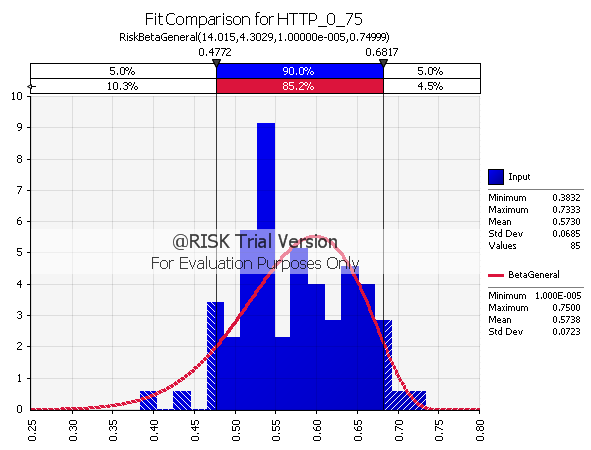
\includegraphics[scale=0.70]{HTTP_0_75_Beta_Graph.png}
\centering
\end{figure}
\begin{figure}[htbp]
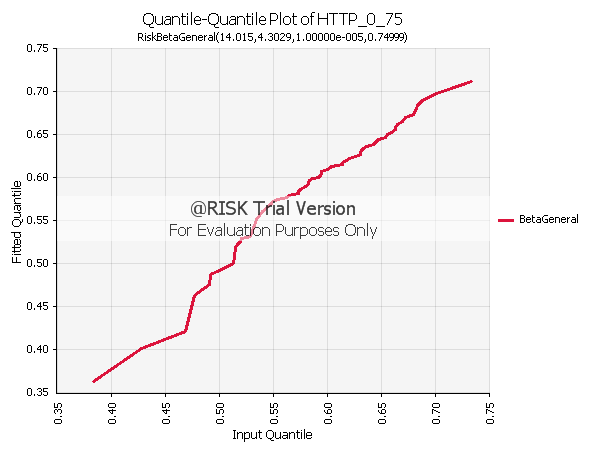
\includegraphics[scale=0.70]{HTTP_0_75_Beta_QQ.png}
\centering
\end{figure}
\begin{figure}[htbp]
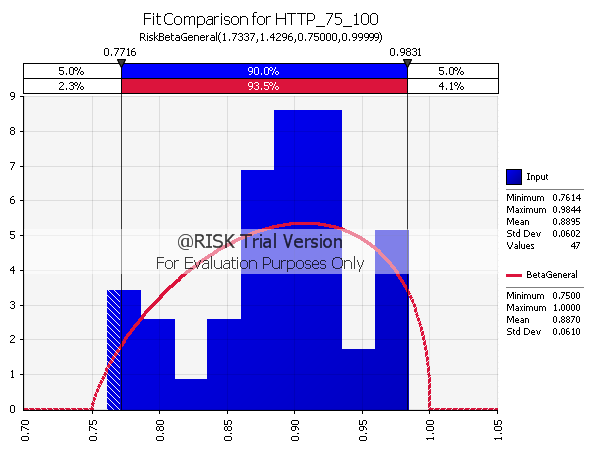
\includegraphics[scale=0.70]{HTTP_75_100_Beta_Graph.png}
\centering
\end{figure}
\begin{figure}[htbp]
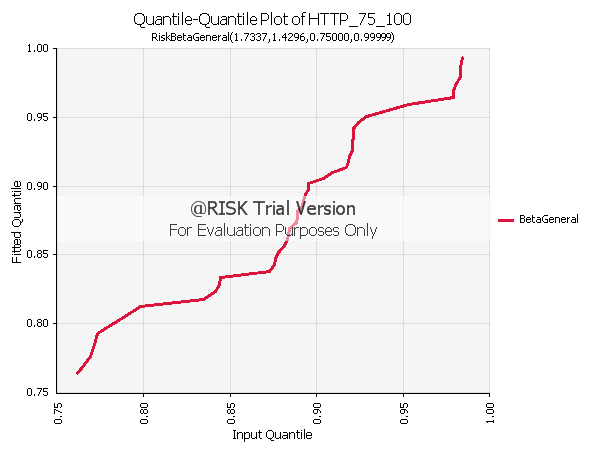
\includegraphics[scale=0.70]{HTTP_75_100_Beta_QQ.png}
\centering
\end{figure}
\begin{figure}[htbp]
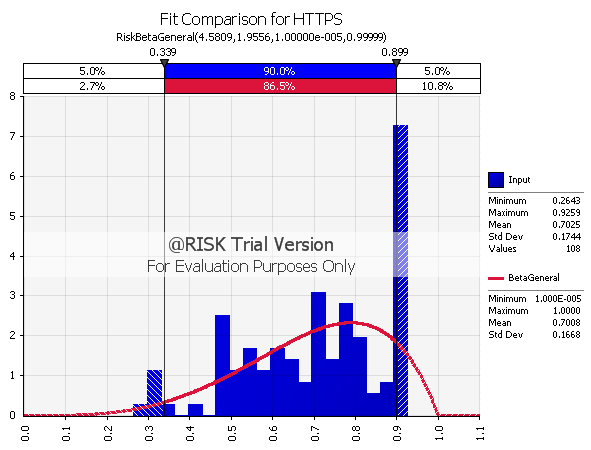
\includegraphics[scale=0.70]{HTTPS_Beta_Graph.png}
\centering
\end{figure}
\begin{figure}[htbp]
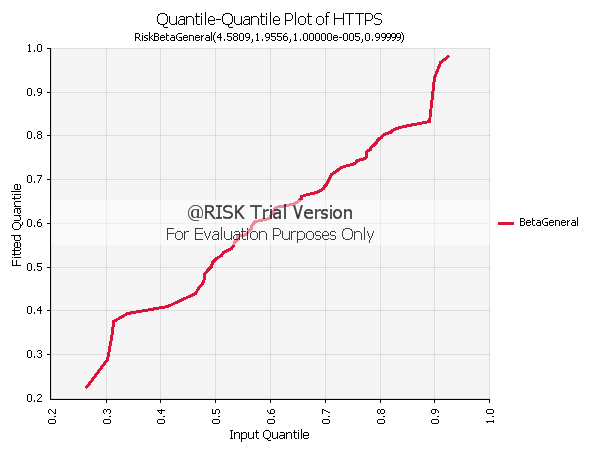
\includegraphics[scale=0.70]{HTTPS_Beta_QQ.png}
\centering
\end{figure}

\end{document}
